
\documentclass[compress,aspectratio=43]{beamer}

\usepackage{fontspec}
\usepackage{polyglossia}
\setmainlanguage{english}
\usepackage[english]{isodate}
\isodate
\usepackage{multicol}
\usepackage{feynmp-auto}
\usepackage{siunitx}
\sisetup{separate-uncertainty}
\usepackage{booktabs}
\usepackage{biblatex}
\addbibresource{main.bib}

\usetheme{vertex}

\linespread{1.3}

\newcommand{\beginbackup}{
   \newcounter{framenumbervorappendix}
   \setcounter{framenumbervorappendix}{\value{framenumber}}
}
\newcommand{\backupend}{
   \addtocounter{framenumbervorappendix}{-\value{framenumber}}
   \addtocounter{framenumber}{\value{framenumbervorappendix}} 
}

\title{Search for $B\to D\mu\mu$}
\subtitle{Theory and Analysis outline}
\date{\today}
\institute{Very Rare Decays WG Meeting}
\author[Igor Babuschkin]{\small \textbf{Igor Babuschkin} \and Julian Wishahi \and Alex Shires \and Johannes Albrecht}

\begin{document}

\maketitle

\begin{frame}{The decay $B^0\to\overline{D}^0\mu^+\mu^-$}
  \centering
  \begin{columns}
    \begin{column}{0.35\textwidth}
      \begin{fmffile}{b2dmumu}
        \centering
        \unitlength=1mm
        \begin{fmfgraph*}(40, 25)
          \fmfcmd{%
            vardef cross_bar (expr p, len, ang) =
            ((-len/2,0)--(len/2,0))
              rotated (ang + angle direction length(p)/2 of p)
              shifted point length(p)/2 of p
            enddef;
            style_def crossed_before expr p =
              cdraw p;
              cfill (harrow (p, .4));
              ccutdraw cross_bar (p, 4mm, 45);
              ccutdraw cross_bar (p, 4mm, -45)
            enddef;
            style_def crossed_after expr p =
              cdraw p;
              cfill (harrow (p, .9));
              ccutdraw cross_bar (p, 4mm, 45);
              ccutdraw cross_bar (p, 4mm, -45)
            enddef;
            style_def crossed_wiggly expr p =
              cdraw (wiggly p);
              ccutdraw cross_bar (p, 4mm, 45);
              ccutdraw cross_bar (p, 4mm, -45)
            enddef; }
          \fmfleft{i1,i2}
          \fmfright{o1,o2}
          \fmf{crossed_after}{v1,i1}
          \fmf{crossed_before}{o1,v1}
          \fmf{crossed_before}{i2,v2}
          \fmf{crossed_after}{v2,o2}
          \fmf{boson,label=$W$}{v1,v2}
          \fmfv{label=$b$}{i1}
          \fmfv{label=$c$}{o1}
          \fmfv{label=$d$}{i2}
          \fmfv{label=$u$}{o2}
        \end{fmfgraph*}

        \centering
        \vspace{3em}
        \begin{fmfgraph*}(20, 15)
          \fmfleft{i1}
          \fmfright{o1,o2}
          \fmf{photon}{i1,v1}
          \fmf{fermion}{o1,v1,o2}
          \fmfv{label=$\gamma/Z^0$,decoration.size=0.2w,decoration.shape=cross}{i1}
          \fmfv{label=$\mu$}{o2}
          \fmfv{label=$\mu$}{o1}
        \end{fmfgraph*}

      \end{fmffile}
    \end{column}
    \begin{column}{0.70\textwidth}
      \begin{itemize}
        \item $W$ exchange (no penguin loop)
        \item Two conflicting theoretical predictions:
        \item Evans et al. [1999] ($q^2 > \SI{1}{GeV^2}$)\\ $\mathrm{BR}(B^0\to \overline{D}^0 e^+e^-) = 2.6\times10^{-9}$
        \item Kim et al. [2011] ($q^2 \in [1,5]\,\si{GeV^2}$) \\ $\mathrm{BR}(B^0\to \overline{D}^0 \mu^+\mu^-) = \left(9.7^{+4.2}_{-3.2}\right)\times10^{-6}$
      \end{itemize}
    \end{column}
  \end{columns}
\end{frame}

\begin{frame}{Evans et al.}
  \begin{itemize}
    \item Use effective field theory approach to separate decay into short/long distance interactions
    \item In absence of lattice QCD calculations, matrix elements $β$ and $β_8$ are approximated
    \item BR for $B^0\to D^{(*)0}e^+e^-$ is calculated
    \item Also give predictions for $B^+\to D_{\!(s)}^{\ (*)+}e^+e^-$ (smaller BR) in a different paper
    \item Use these to get an idea of expected yields
  \end{itemize}
\end{frame}

\begin{frame}{Kim et al.}
  \begin{itemize}
    \item Perturbative QCD approach
    \item Make use of model-dependent wave functions to derive result
    \item No mention of calculation by Evans et al.
    \item We should treat this optimistic result with care
  \end{itemize}
\end{frame}

\begin{frame}{Expected number of candidates}
  \begin{columns}
    \begin{column}{0.4\textwidth}
      \begin{itemize}
        \item $\mathcal{L} = \SI{3.189}{\per\femto\barn}$
        \item $σ_{b\overline{b}} = \SI{295 \pm 29}{\micro\barn}$
        \item $f_d \approx \num{0.4}$
        \item $ε_\text{geom} \approx \num{0.15}$
        \item $ε_\text{trig} \approx \num{0.8}$
        \item $ε_\text{strip} \approx \num{0.2}$
      \end{itemize}
    \end{column}
    \begin{column}{0.7\textwidth}
      \begin{itemize}
        %\item $\mathrm{BR}(D^{0}\to K^-\pi^+) = \SI{3.87 \pm 0.05}{\percent}$
        %\item $\mathrm{BR}(D^+\to K^-\pi^+\pi^+) = \SI{9.13 \pm 0.19}{\percent}$
        %\item $\mathrm{BR}(D_s^+\to K^+K^-\pi^+) = \SI{5.49 \pm 0.27}{\percent}$
        %\item $\mathrm{BR}(D^{*0} \to D^0\pi^0) = \SI{61.9 \pm 2.9}{\percent}$
        %\item $\mathrm{BR}(D^{*+} \to D^0\pi^+) = \SI{67.7 \pm 0.5}{\percent}$
        %\item $\mathrm{BR}(D_s^{+*}\to D_s^+\pi^0) = \SI{5.8 \pm 0.7}{\percent}$
        \item Use conservative theory estimates (Evans, \cite{evans1}\cite{evans2}) for $B$ decay BRs
        \item (All $B$ BRs for $q^2 > \SI{1}{GeV^2}$)
        \item Take $D$ branching fractions from PDG
      \end{itemize}
    \end{column}
  \end{columns}
  Calculate yields not including selection efficiencies:
  \begin{equation*}
    N = \mathcal{L}\,\sigma_{b\overline{b}}\,2 f_d\,ε_\text{geom}\,ε_\text{trig}\,ε_\text{strip}\,\text{BR}_B\,\text{BR}_D
  \end{equation*}
\end{frame}

\begin{frame}[shrink=20]{Expected number of candidates (cont.)}
  \begin{itemize}
    \item BRs used: Evans (\cite{evans1}\cite{evans2})
  \end{itemize}
  \centering
  \begin{tabular}{l S S}
    \toprule
    Decay & {\text{Predicted BR}} & {\text{Expected yield}} \\
    \midrule
    $\mathbf{B^0\to \overline{D}^0\mu\mu}$ & 2.6e-9 & 1.8 \\
    $B^0\to \overline{D}^{*0}\mu\mu$ & 1.4e-8 & 6.1 \\
    $B^+\to D^+\mu\mu$ & 2.5e-12 & 0.41e-2 \\
    $\mathbf{B^+\to D^{+*}\mu\mu}$ & 1.0e-11 & 0.48e-2 \\
    $\mathbf{B^+\to D_s^+\mu\mu}$ & 4.3e-11 & 0.17e-2 \\
    $B^+\to D_s^{+*}\mu\mu$ & 2.0e-10 & 0.12e-1 \\
    \bottomrule
  \end{tabular}
  \begin{itemize}
    \item Other interesting possibility: $B_c \to D_s^+\mu\mu$
      \begin{itemize}
        \item but BR $\sim 10^{-7}$ (Ebert\cite{ebert})
        \item investigate if measurement is feasible
      \end{itemize}
    \item Also: Most resonant modes ($D J/\psi$) not yet observed
  \end{itemize}
\end{frame}

\begin{frame}{Trigger and Stripping}
  \begin{itemize}
    \item Use standard muon trigger lines
    \item Stripping line: \texttt{StrippingB2XMuMu\_Line}
      \begin{itemize}
        \item Final states with $2\mu$ and additionally $X=\phi,J/\psi,K,K^*,D^{*+},D,...$
        \item Cuts: mostly loose vertex quality cuts
      \end{itemize}
  \end{itemize}
\end{frame}

\begin{frame}{Preparation: Blind signal region, Remove $J/\psi$}
  \centering
  \includegraphics[width=0.75\textwidth,page=80]{../../../plots/select.pdf}
\end{frame}

\begin{frame}{Preselection}
  \begin{itemize}
    \item {\small Cut on PID variables and \texttt{isMuonLoose} to select Kaon/Pion:}
  \end{itemize}
  \centering
  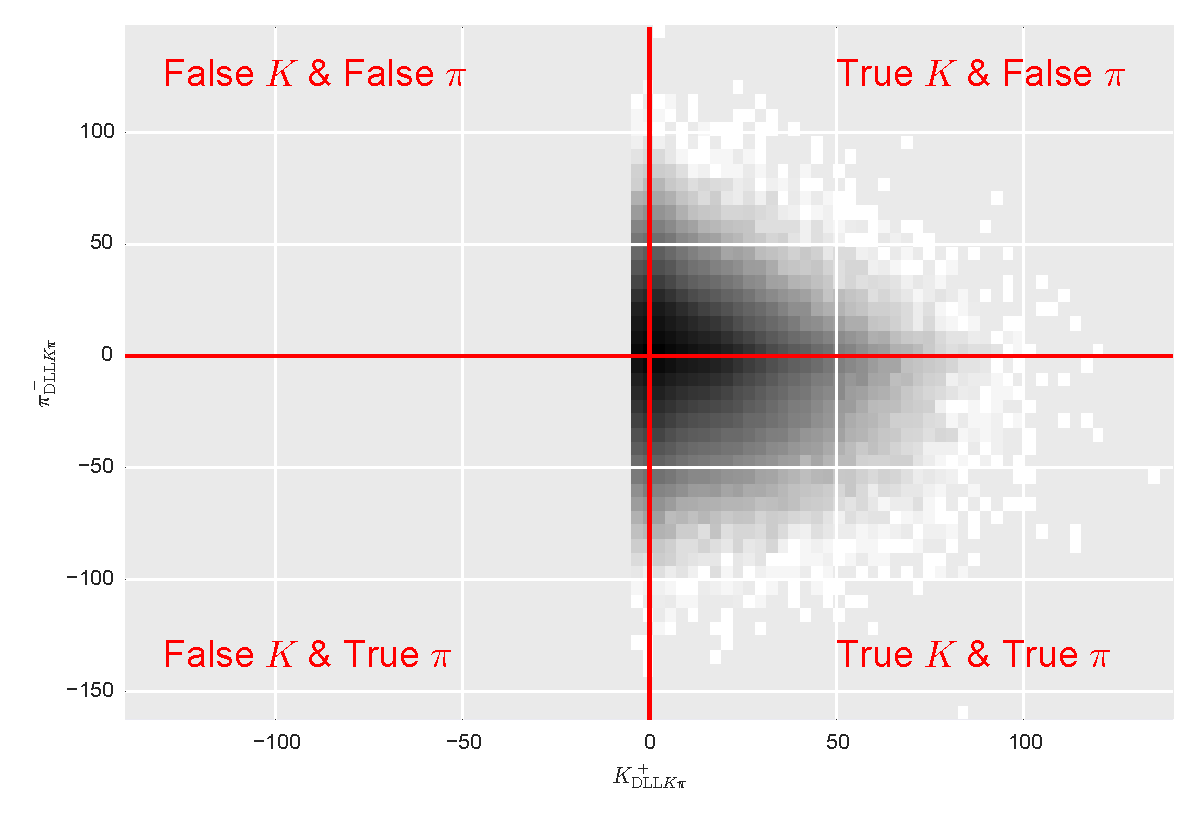
\includegraphics[width=0.65\textwidth,trim=0 4em 0 0,clip]{../../../plots/pid_plot.pdf}
  \begin{itemize}
    \item Resampling of PID variables from data in progress
    \item Preselection can be improved: cut on $D^0$ mass?
  \end{itemize}
\end{frame}

\begin{frame}[shrink=20]{Multivariate selection: variables}
  \begin{itemize}
    \item Signal proxy: $B^0\to \overline{D}^0\mu\mu$ MC12
    \item Background proxy: Upper $B$ mass sideband
    \item Choice of variables inspired by $B^0\to K^*\mu\mu$ selection
    \item Work planned to optimize this (look at measures beyond BDT importance)
    \item Use Isolation discriminant from $B^0\to K^{*0}\mu\mu$ analysis
  \end{itemize}
  \centering
  \includegraphics[trim=0 4em 0 8em,clip,width=0.65\textwidth]{../../../plots/correlation.pdf}
\end{frame}

\begin{frame}[shrink=20]{Multivariate selection: cross-validation, ROC curves}
  \begin{itemize}
    \item Use $k$-fold validation to assess quality of classifier (BDT)
    \item ROC curves for each of the $k=5$ test samples
  \end{itemize}

  \centering
  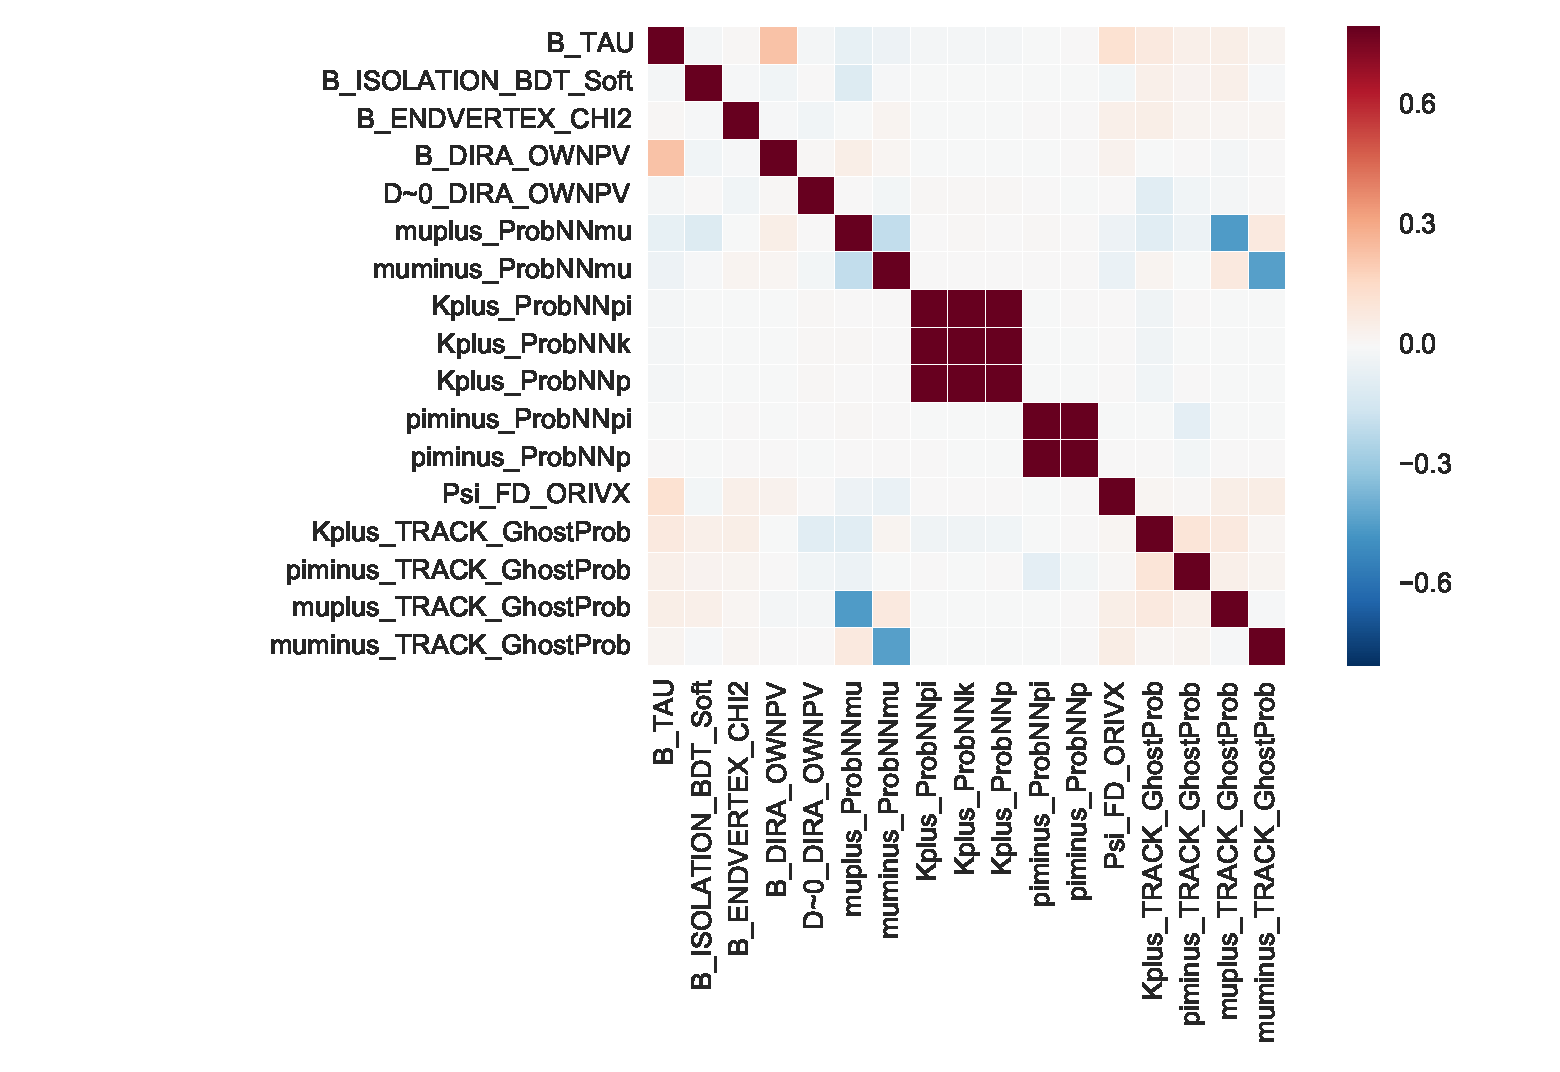
\includegraphics[width=0.60\textwidth,page=1]{../../../plots/classifier.pdf}

  \begin{itemize}
    \item It's strange that these deviate significantly $\rightarrow$ needs to be understood
  \end{itemize}
\end{frame}

\begin{frame}{Multivariate selection: Cuts on classifier}
  \centering
  \includegraphics[width=0.8\textwidth]{../../../plots/classifier_mass.pdf}
  \begin{itemize}
    \item {\small Classifier seems to be correlated with mass $\rightarrow$ needs to be fixed}
  \end{itemize}
\end{frame}

\begin{frame}{Suspected physical background: $B^0\to K^+\pi^-\mu\mu$}
  \begin{itemize}
      \item Nonresonant contribution is a problem for $B^0\to J/\psi \overline{D}^0$
      \begin{itemize}
        \item See note \texttt{LHCB-ANA-2012-111}
        \item How to deal with this? $D^0$ lifetime cut removes a lot of signal
        \item Idea: Include $D^0$ mass (and optionally $D^0$ decay time) into fit 
        \item Use $B^0\to K^+\pi^-\mu\mu$ (exists) to determine shape
      \end{itemize}
    \item Started to investigate with toy MC (simultaneous fit)
  \end{itemize}
  \centering
  \includegraphics[width=0.5\textwidth,trim=0 0 0 4em,clip]{../../../plots/fit_bmass.pdf}
  \includegraphics[width=0.5\textwidth,trim=0 0 0 4em,clip]{../../../plots/fit_dmass.pdf}
\end{frame}

\begin{frame}{Measurement of branching fraction}
  Needed are:
  \begin{itemize}
    \item trigger efficiency (use TISTOS on control channel)
    \item stripping efficiency (MC)
    \item LHCb acceptance efficiency (MC)
    \item preselection efficiency (use PIDCalib/Resampling?)
    \item selection efficiency of BDT
  \end{itemize}
  $\Rightarrow$ Use signal yield and efficiencies to derive BR estimate.
  \begin{itemize}
    \item Choose normalization/control channel:
      \begin{itemize}
        \item $B^0\to K^{*0}\mu^+\mu^-$ $\Rightarrow$ Similar behaviour
        \item $B^0 \to K^{*0}J\!/\!\psi$ $\Rightarrow$ Larger statistics
      \end{itemize}
  \end{itemize}
\end{frame}

\begin{frame}[shrink=20]{Outlook}
  \begin{itemize}
    \item Analysis of $B\to D \mu^+\mu^-$ has started
    \item Many possible final states to look at
    \item Restrict to most promising ones:
    \begin{itemize}
      \item $B^0 \to \overline{D}^0\mu\mu$ is progressing
      \item $B^+ \to D^{+*}\mu\mu$,\ $B^+ \to D_s^{+}\mu\mu$,\ $B_c^+\to D_s^+\mu\mu$ need simulation
      \item Also look at currently unobserved resonant modes (same dataset)
      \item Decfiles for nonresonant modes ($\mu\mu$) all released. Need to look into resonant ($J/\psi$)
    \end{itemize}
    \item We would like to request moderate signal MC samples for these channels (resonant/nonresonant)\\ 
      $\Rightarrow$ Use these to define exactly which channels should be covered
  \end{itemize}
  Judging from theory prediction (Evans): Expect to set limits
  \begin{itemize}
    \item But: The BR could be underestimated!
  \end{itemize}
\end{frame}

\begin{frame}[shrink=20]{Bibliography}
  \small
  \printbibliography
\end{frame}

\appendix
\beginbackup

\begin{frame}{Test for overtraining}
  \centering
  \includegraphics[width=0.7\textwidth,page=2]{../../../plots/classifier.pdf}
\end{frame}
\backupend

\end{document}

